% Editable source for result.pdf, written by make_figures.py from run_github_39335956567/panel/result.json
\documentclass[tikz,border=6pt]{standalone}
\usepackage[T1]{fontenc}
\begin{document}
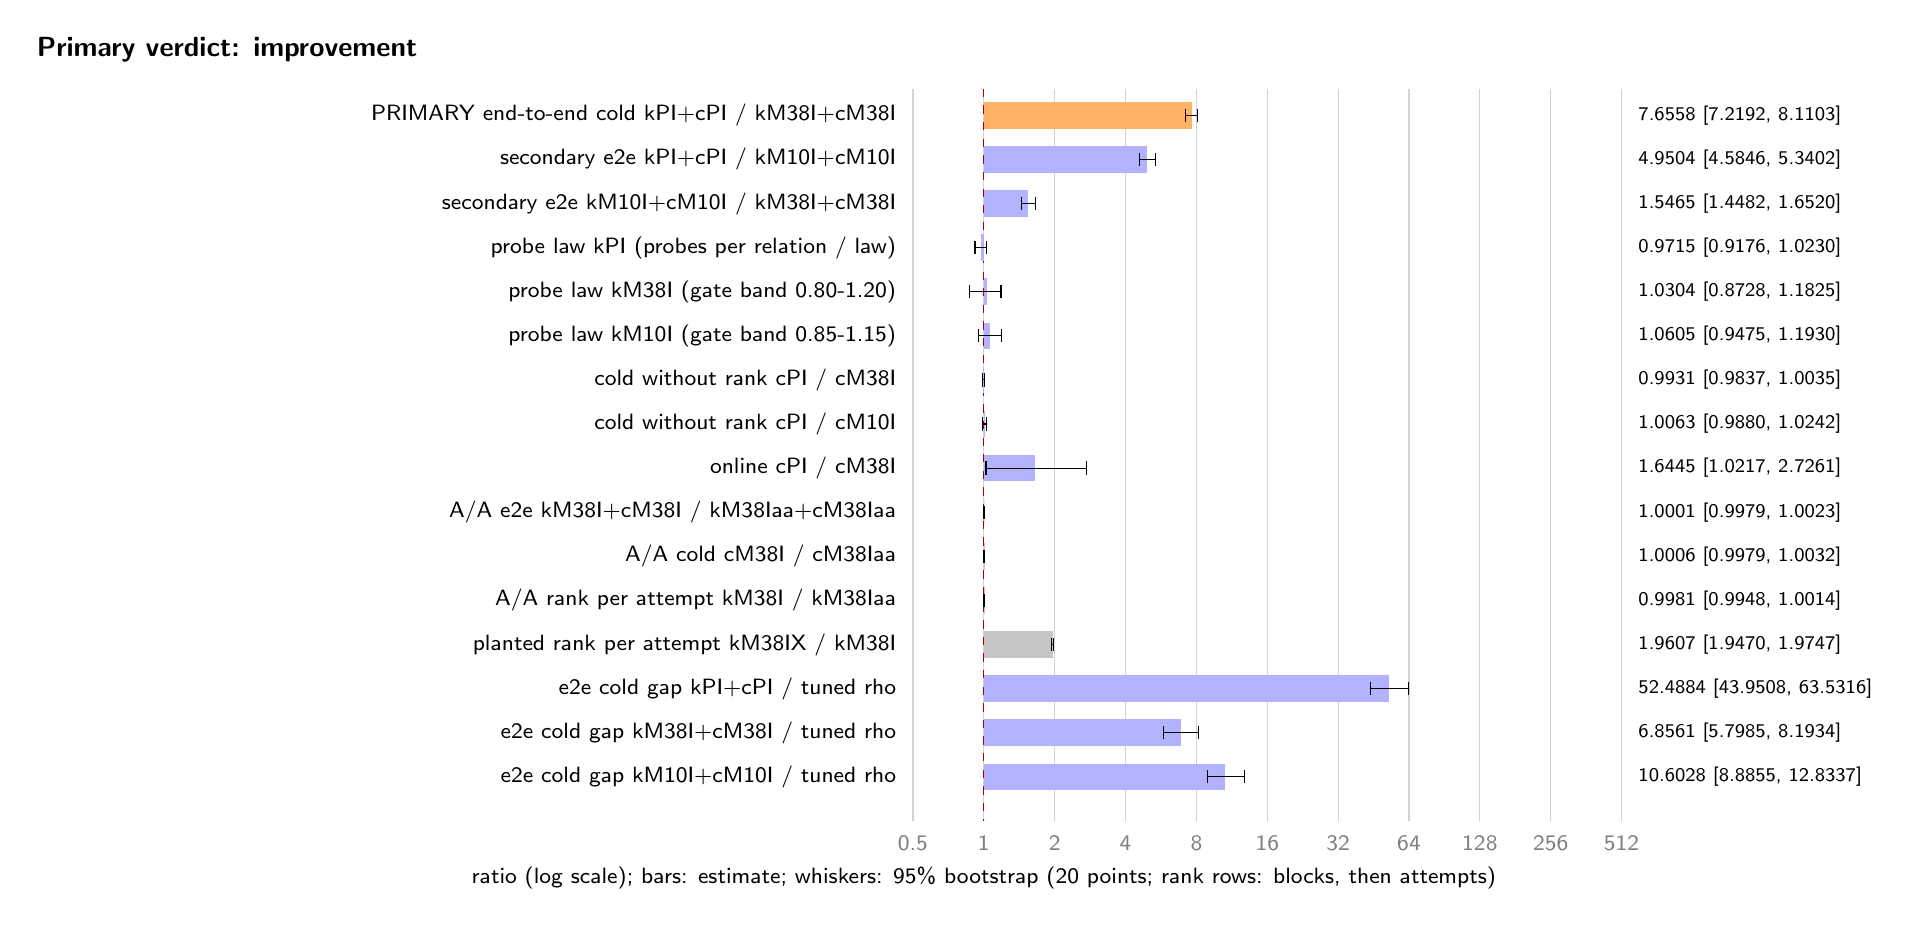
\begin{tikzpicture}[font=\sffamily\footnotesize,x=9mm,y=-5.6mm]
\draw[gray!35] (-1.0000,-0.6) -- (-1.0000,16); \node[gray] at (-1.0000,16.5) {0.5};
\draw[gray!35] (0.0000,-0.6) -- (0.0000,16); \node[gray] at (0.0000,16.5) {1};
\draw[gray!35] (1.0000,-0.6) -- (1.0000,16); \node[gray] at (1.0000,16.5) {2};
\draw[gray!35] (2.0000,-0.6) -- (2.0000,16); \node[gray] at (2.0000,16.5) {4};
\draw[gray!35] (3.0000,-0.6) -- (3.0000,16); \node[gray] at (3.0000,16.5) {8};
\draw[gray!35] (4.0000,-0.6) -- (4.0000,16); \node[gray] at (4.0000,16.5) {16};
\draw[gray!35] (5.0000,-0.6) -- (5.0000,16); \node[gray] at (5.0000,16.5) {32};
\draw[gray!35] (6.0000,-0.6) -- (6.0000,16); \node[gray] at (6.0000,16.5) {64};
\draw[gray!35] (7.0000,-0.6) -- (7.0000,16); \node[gray] at (7.0000,16.5) {128};
\draw[gray!35] (8.0000,-0.6) -- (8.0000,16); \node[gray] at (8.0000,16.5) {256};
\draw[gray!35] (9.0000,-0.6) -- (9.0000,16); \node[gray] at (9.0000,16.5) {512};
\draw[red!70!black,dashed] (0,-0.6) -- (0,16);
\node at (0,17.3) {ratio (log scale); bars: estimate; whiskers: 95\% bootstrap (20 points; rank rows: blocks, then attempts)};
\node[anchor=west,font=\sffamily\bfseries] at (-13.5,-1.5) {Primary verdict: improvement};
\node[anchor=east] at (-1.1000,0) {PRIMARY end-to-end cold kPI+cPI / kM38I+cM38I};
\fill[orange!60] (0,-0.300000) rectangle (2.9365,0.300000);
\draw (2.8518,0) -- (3.0197,0); \draw (2.8518,-0.150000) -- (2.8518,0.150000); \draw (3.0197,-0.150000) -- (3.0197,0.150000);
\node[anchor=west,font=\sffamily\scriptsize] at (9.1000,0) {7.6558 [7.2192, 8.1103]};
\node[anchor=east] at (-1.1000,1) {secondary e2e kPI+cPI / kM10I+cM10I};
\fill[blue!30] (0,0.700000) rectangle (2.3076,1.300000);
\draw (2.1968,1) -- (2.4169,1); \draw (2.1968,0.850000) -- (2.1968,1.150000); \draw (2.4169,0.850000) -- (2.4169,1.150000);
\node[anchor=west,font=\sffamily\scriptsize] at (9.1000,1) {4.9504 [4.5846, 5.3402]};
\node[anchor=east] at (-1.1000,2) {secondary e2e kM10I+cM10I / kM38I+cM38I};
\fill[blue!30] (0,1.700000) rectangle (0.6290,2.300000);
\draw (0.5343,2) -- (0.7242,2); \draw (0.5343,1.850000) -- (0.5343,2.150000); \draw (0.7242,1.850000) -- (0.7242,2.150000);
\node[anchor=west,font=\sffamily\scriptsize] at (9.1000,2) {1.5465 [1.4482, 1.6520]};
\node[anchor=east] at (-1.1000,3) {probe law kPI (probes per relation / law)};
\fill[blue!30] (0,2.700000) rectangle (-0.0418,3.300000);
\draw (-0.1241,3) -- (0.0328,3); \draw (-0.1241,2.850000) -- (-0.1241,3.150000); \draw (0.0328,2.850000) -- (0.0328,3.150000);
\node[anchor=west,font=\sffamily\scriptsize] at (9.1000,3) {0.9715 [0.9176, 1.0230]};
\node[anchor=east] at (-1.1000,4) {probe law kM38I (gate band 0.80-1.20)};
\fill[blue!30] (0,3.700000) rectangle (0.0433,4.300000);
\draw (-0.1963,4) -- (0.2418,4); \draw (-0.1963,3.850000) -- (-0.1963,4.150000); \draw (0.2418,3.850000) -- (0.2418,4.150000);
\node[anchor=west,font=\sffamily\scriptsize] at (9.1000,4) {1.0304 [0.8728, 1.1825]};
\node[anchor=east] at (-1.1000,5) {probe law kM10I (gate band 0.85-1.15)};
\fill[blue!30] (0,4.700000) rectangle (0.0847,5.300000);
\draw (-0.0778,5) -- (0.2546,5); \draw (-0.0778,4.850000) -- (-0.0778,5.150000); \draw (0.2546,4.850000) -- (0.2546,5.150000);
\node[anchor=west,font=\sffamily\scriptsize] at (9.1000,5) {1.0605 [0.9475, 1.1930]};
\node[anchor=east] at (-1.1000,6) {cold without rank cPI / cM38I};
\fill[blue!30] (0,5.700000) rectangle (-0.0100,6.300000);
\draw (-0.0238,6) -- (0.0051,6); \draw (-0.0238,5.850000) -- (-0.0238,6.150000); \draw (0.0051,5.850000) -- (0.0051,6.150000);
\node[anchor=west,font=\sffamily\scriptsize] at (9.1000,6) {0.9931 [0.9837, 1.0035]};
\node[anchor=east] at (-1.1000,7) {cold without rank cPI / cM10I};
\fill[blue!30] (0,6.700000) rectangle (0.0090,7.300000);
\draw (-0.0174,7) -- (0.0345,7); \draw (-0.0174,6.850000) -- (-0.0174,7.150000); \draw (0.0345,6.850000) -- (0.0345,7.150000);
\node[anchor=west,font=\sffamily\scriptsize] at (9.1000,7) {1.0063 [0.9880, 1.0242]};
\node[anchor=east] at (-1.1000,8) {online cPI / cM38I};
\fill[blue!30] (0,7.700000) rectangle (0.7177,8.300000);
\draw (0.0309,8) -- (1.4469,8); \draw (0.0309,7.850000) -- (0.0309,8.150000); \draw (1.4469,7.850000) -- (1.4469,8.150000);
\node[anchor=west,font=\sffamily\scriptsize] at (9.1000,8) {1.6445 [1.0217, 2.7261]};
\node[anchor=east] at (-1.1000,9) {A/A e2e kM38I+cM38I / kM38Iaa+cM38Iaa};
\fill[gray!45] (0,8.700000) rectangle (0.0002,9.300000);
\draw (-0.0031,9) -- (0.0034,9); \draw (-0.0031,8.850000) -- (-0.0031,9.150000); \draw (0.0034,8.850000) -- (0.0034,9.150000);
\node[anchor=west,font=\sffamily\scriptsize] at (9.1000,9) {1.0001 [0.9979, 1.0023]};
\node[anchor=east] at (-1.1000,10) {A/A cold cM38I / cM38Iaa};
\fill[gray!45] (0,9.700000) rectangle (0.0009,10.300000);
\draw (-0.0030,10) -- (0.0046,10); \draw (-0.0030,9.850000) -- (-0.0030,10.150000); \draw (0.0046,9.850000) -- (0.0046,10.150000);
\node[anchor=west,font=\sffamily\scriptsize] at (9.1000,10) {1.0006 [0.9979, 1.0032]};
\node[anchor=east] at (-1.1000,11) {A/A rank per attempt kM38I / kM38Iaa};
\fill[gray!45] (0,10.700000) rectangle (-0.0028,11.300000);
\draw (-0.0075,11) -- (0.0020,11); \draw (-0.0075,10.850000) -- (-0.0075,11.150000); \draw (0.0020,10.850000) -- (0.0020,11.150000);
\node[anchor=west,font=\sffamily\scriptsize] at (9.1000,11) {0.9981 [0.9948, 1.0014]};
\node[anchor=east] at (-1.1000,12) {planted rank per attempt kM38IX / kM38I};
\fill[gray!45] (0,11.700000) rectangle (0.9714,12.300000);
\draw (0.9612,12) -- (0.9817,12); \draw (0.9612,11.850000) -- (0.9612,12.150000); \draw (0.9817,11.850000) -- (0.9817,12.150000);
\node[anchor=west,font=\sffamily\scriptsize] at (9.1000,12) {1.9607 [1.9470, 1.9747]};
\node[anchor=east] at (-1.1000,13) {e2e cold gap kPI+cPI / tuned rho};
\fill[blue!30] (0,12.700000) rectangle (5.7139,13.300000);
\draw (5.4578,13) -- (5.9894,13); \draw (5.4578,12.850000) -- (5.4578,13.150000); \draw (5.9894,12.850000) -- (5.9894,13.150000);
\node[anchor=west,font=\sffamily\scriptsize] at (9.1000,13) {52.4884 [43.9508, 63.5316]};
\node[anchor=east] at (-1.1000,14) {e2e cold gap kM38I+cM38I / tuned rho};
\fill[blue!30] (0,13.700000) rectangle (2.7774,14.300000);
\draw (2.5357,14) -- (3.0345,14); \draw (2.5357,13.850000) -- (2.5357,14.150000); \draw (3.0345,13.850000) -- (3.0345,14.150000);
\node[anchor=west,font=\sffamily\scriptsize] at (9.1000,14) {6.8561 [5.7985, 8.1934]};
\node[anchor=east] at (-1.1000,15) {e2e cold gap kM10I+cM10I / tuned rho};
\fill[blue!30] (0,14.700000) rectangle (3.4064,15.300000);
\draw (3.1515,15) -- (3.6819,15); \draw (3.1515,14.850000) -- (3.1515,15.150000); \draw (3.6819,14.850000) -- (3.6819,15.150000);
\node[anchor=west,font=\sffamily\scriptsize] at (9.1000,15) {10.6028 [8.8855, 12.8337]};
\end{tikzpicture}
\end{document}
